\section{Results}
\textcolor{blue}{Speaking about the three methods on with tweet-embeddings}

As the two convolutional neural nets were giving the best results, they were trained for longer times using the full dataset provided. After a few hours of training, some results appeared [FIG. \ref{plot:CNNaccuracy}]. The figure display the training accuracy of the two models. The first one was not using the dropout method as opposed as the second one. 96\% of the data are kept for training the neural net and 4\% is used to validate the predictions. Each time all the train data are learned by the neural net, the test sample is evaluated. These results corresponds to the cross on the figure. The convolutional neural net using dropout was faster to train, as expected. And it was giving more significant results. So after a while the training of the other network was stop, and only the one with dropout was kept. 

\label{sec:results}
\begin{figure}[h!]
\centering
	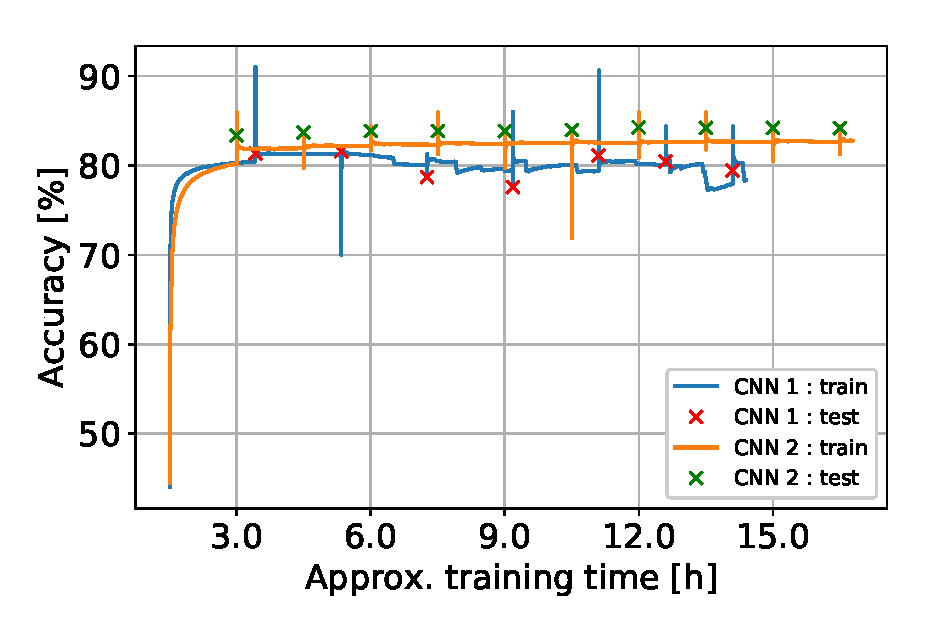
\includegraphics[scale=0.6]{CNNaccuracy} 
\caption{Training of the two convolutional neural nets. The first one does not use ``dropout'' as opposed as the second one.}
\label{plot:CNNaccuracy}
\end{figure}
\FloatBarrier


\begin{table}[h]
  \centering
  \begin{tabular}[c]{lllll}
    Input format&Model&Accuracy&Precision&Recall\\
    \hline
    Tweet-embed.&Logistic regression & 60.60 &    60.84   & 60.64  \\
    Tweet-embed.&SVM             & 61.96    &   63.69     & 62.05   \\
    Tweet-embed.&Neural network & 65.45	& 67.04	& 65.53	 \\
    Word-embed.&CNN w.o. dropout &  81.12  & 81.80	& 81.75	 \\
    Word-embed.&CNN w. dropout & 84.29 & 84.79 & 84.74 
    
  \end{tabular}
  \caption{Classification performances using local hold-out testing, for various input data formats.All the data are given in \%}
  \label{tab:results}
\end{table}


